% PLEASE USE THIS FILE AS A TEMPLATE
% Check file iosart2c.tex for more examples
%
% Journal:
%   Journal of Ambient Intelligence and Smart Environments (jaise)
%   Web Intelligence and Agent Systems: An International Journal (wias)
%   Semantic Web: Interoperability, Usability, Applicability (SW)
% IOS Press
% Latex 2e

% options: jaise|wias|sw
% add. options: [seceqn,secfloat,secthm,crcready,onecolumn]

\documentclass{iosart2c}

%\documentclass[sw]{iosart2c}
%\documentclass[wias]{iosart2c}
%\documentclass[jaise]{iosart2c}

\usepackage[T1]{fontenc}
\usepackage{times}%
\usepackage{natbib}% for bibliography sorting/compressing
%\usepackage{amsmath}
%\usepackage{endnotes}
\usepackage{graphicx}
\usepackage[lofdepth,lotdepth]{subfig}
\usepackage[activate=compatibility]{microtype}


%%%%%%%%%%% Put your definitions here
\usepackage[utf8]{inputenc}
\usepackage[hyphens]{url}
\usepackage{verbatim} 
\usepackage[pdftex,urlcolor=black,colorlinks=true,linkcolor=black,citecolor=black,draft]{hyperref}
\def\sectionautorefname{Section}
\def\subsectionautorefname{Subsection}
\def\tabularautorefname{Table}
\def\tableautorefname{Table}
\usepackage{listings}
\usepackage{textcomp}
\lstset{
        basicstyle=\ttfamily\scriptsize,
        upquote=true,
        showspaces=false,
        showstringspaces=false,
        showtabs=false,
        tabsize=2,
        frame=none,
        breaklines,
        numbers=none,
        framexleftmargin=2mm,
        xleftmargin=2mm,
        captionpos=b
}
\usepackage{caption}
\DeclareCaptionFormat{listing}{\footnotesize#1#2#3}
\captionsetup[lstlisting]{format=listing}

% todo macro
\usepackage{color}
\newcommand{\todo}[1]{\noindent\textcolor{red}{{\bf \{TODO}: #1{\bf \}}}}

% table captions
\newcommand{\tablecaption}[1]{%
  \\[1em]%
  \refstepcounter{table}%
  Table \arabic{table}: #1%
}

%% Define a new 'smallurl' style for the package that will use a smaller font.
\makeatletter
\def\url@smallurlstyle{%
  \@ifundefined{selectfont}{\def\UrlFont{\sf}}{\def\UrlFont{\scriptsize\ttfamily}}}
\makeatother
%% Now actually use the newly defined style.
\urlstyle{smallurl}
\newcommand{\nofootnote}[1]{~#1}

%%%%%%%%%%% End of definitions

\pubyear{0000}
\volume{0}
\firstpage{1}
\lastpage{1}

\begin{document}

\begin{frontmatter}

\pretitle{What'chu talkin' about, Willis?}
\title{A consumer's look on Facebook and Twitter~-- What do people read and where?}
\runningtitle{A consumer's look on Facebook and Twitter~-- What do people read and where?}

% Two or more authors:
\author[A]{\fnms{Thomas} \snm{Steiner}},
\author[B]{\fnms{Ruben} \snm{Verborgh}},
\author[A]{\fnms{Arnaud} \snm{Brousseau}\thanks{A. Brousseau was an intern at Google Germany GmbH at the time of writing.}},
\author[C]{\fnms{Raphaël} \snm{Troncy}},
\author[B]{\fnms{Rik} \snm{Van de Walle}},
\author[D]{\fnms{Joaquim} \snm{Gabarró Vallés}}

\runningauthor{T. Steiner, R. Verborgh, A. Brousseau, R. Troncy, \textit{et al.}}

\address[A]{Google Germany GmbH, ABC-Str. 19, 20354 Hamburg, Germany,\\
E-mail: tomac@google.com, arnaud.brousseau@gmail.com}
\address[B]{Ghent University -- IBBT, ELIS, Multimedia Lab, Gaston Crommenlaan 8/201, 9050 Ghent, Belgium,\\
E-mail: ruben.verborgh@ugent.be, rik.vandewalle@ugent.be}
\address[C]{EURECOM, Sophia Antipolis, France\\
E-mail: raphael.troncy@eurecom.fr}
\address[D]{Universitat Polit\`{e}cnica de Catalunya, Department LSI, 08034 Barcelona, Spain,\\
E-mail: gabarro@lsi.upc.edu}

\begin{abstract}
With the ever-growing influence of social networks, social media mining becomes more and more important as a source for responses to all sorts of questions.
\textit{``Do people like product~X?''};
\textit{``What do people think of a new law proposal~Y?''};
\textit{``Will candidate~A or candidate~B win the elections?''}.
These are just some sample questions where social networks can substantially contribute to answers.
In this paper, we propose a paradigm shift in order to find responses.
Where traditional social media mining focuses exclusively on the producer side of microposts, we focus on the consumer side, that is, on the readers of microposts.
Traditional social media mining retrieves its data through official Application Programming Interfaces (APIs).
In contrast, our approach works through accessing its data directly from the social network users' timeline when they visit the social network via a Web browser.
In comparison to social data retrieved via APIs, the social data retrieved via our approach is more sparse, however, we argue in the paper that it is of higher quality.
We have implemented browser extensions for the popular social networks Facebook and Twitter.
These extensions perform named entity disambiguation on microposts and, via Web analytics software, enabled us to collect social data over the course of six months.
In the first part of the paper, we present global statistics and a comparison of what topics people are interested in on the two examined social networks.
In the second part, using concrete examples from recent history, we show how additional data gathered through Web analytics software can be used to get fine-grained information on geolocations of centers of interest.
This allows for interesting new kinds of questions to be addressed.
\textit{``Does an event~X cause more reader interest in country~A than in country~B?''};
\textit{``Which continent cares most about a catastrophe~Y?''};
\textit{``Do people in city~Z read about product~P?''}.
Finally, as our approach allows for cross-network social media mining, we can even propose answers for a question like the following:
\textit{``Is my brand~B read more about in region~R on social network~A, or social network~B?''}.
We see our approach not as a replacement of traditional social media mining, but more as an additional perspective that makes sense in certain scenarios, some of which we present in this paper.
\end{abstract}

\begin{keyword}
Social media mining, named entity disambiguation, Web analytics
\end{keyword}

\end{frontmatter}

%%%%%%%%%%% The article body starts:

\section{Introduction} \label{sec:introduction}
\subsection{On Traditional Social Media Mining}
In recent years, social media mining has become an essential tool for marketers, traders, and researchers.
The information people share publicly via so-called \emph{microposts} on social networks harbor tremendous amounts of valuable social data.
Forbes has called the social graph \emph{crude oil} in a recent blog post~\cite{ForbesPost}:
\begin{quotation}
\hspace{-.9em}\hyphenation{complex}
``The point is, crude oil is crude. It is an unrefined and complex natural resource containing many riches. It takes time to figure out what to do with a new crude resource.''
\end{quotation}
Social networks today are very much seen as ``walled gardens'', excellently illustrated by a cartoon by David Simonds~(\autoref{fig:DavidSimonds}).
This network isolatedness reflects on how traditional social media mining is done nowadays.
Common literature typically either focuses on just one network (e.g.,~\cite{russell201121}), or treats the different networks separately (e.g.,~\cite{russell2011mining}).
Traditional social media mining happens (i) based on either term-based search APIs, and/or (ii) based on so-called ``fire hose'' near-realtime streaming APIs, which are both provided by the social networks themselves.
The main difference between (i) and (ii) is that in the prior case terms like the name of a brand or company are \emph{proactively} searched for, whereas in the latter case the social media mining system \emph{reactively} acts upon the occurrence of such terms.

\begin{figure}
\centering
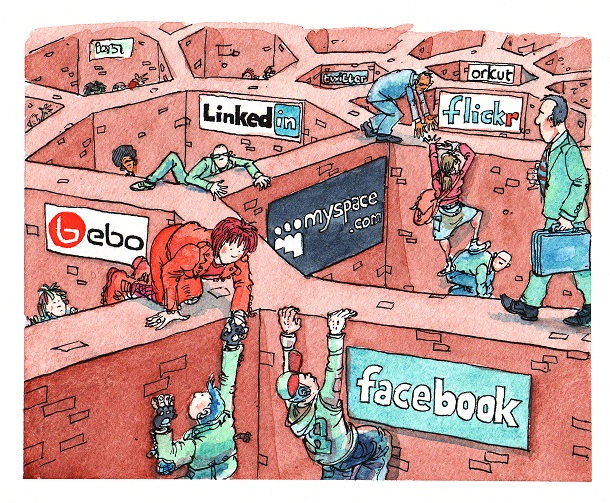
\includegraphics[width=1.0\linewidth,trim=16px 17px 12px 15px,clip]{./resources/davidsimonds.jpg}
\caption{David Simonds illustrates social networks as walled gardens due to their (by design) lock-in effects~\cite{DavidSimonds}.}
\label{fig:DavidSimonds}
\end{figure}

\subsection{Selection of Social Networks and APIs}
In this paper, we consider the popular social networks Facebook~\cite{Facebook} and Twitter~\cite{Twitter}, currently the two globally most important social networks~\cite{comScoreTwitter, comScoreFacebook}.
Traditionally, Twitter is very permissive with its API, as since the beginning of the platform, API-based Twitter clients play a strategic role for the company.
Twitter provides developers with the Twitter Streaming API~\cite{TwitterStreamingAPI}, which allows for high-throughput near-realtime access to various subsets of public and protected Twitter data, at a coverage rate of 1\% (``sprinkler''), 10\% (``garden hose''), or 100\% (``fire hose'') of all Twitter traffic.
Facebook has no such public ``fire hose'' streaming API but supports near-realtime updates via its Graph API~\cite{FacebookRealtimeAPI} to enable applications to subscribe to a limited set of changes in data.
Whenever such a change occurs, Facebook notifies subscribers with a list of changes.
The obvious issue here is that, in order to get a Twitter Streaming API-like experience, one has to subscribe to an impossibly high number of users.
This imbalance in data availability via the respective APIs has an impact on academic publications on social network mining.
While at the World Wide Web Conference 2011 (WWW2011) alone, three Twitter papers based on the Twitter API were published~\cite{Meeder:2011:WKY:1963405.1963479, Romero:2011:DMI:1963405.1963503, Wu:2011:SWT:1963405.1963504}, publications on Facebook typically focus on privacy issues (e.g.,~\cite{liu:settings}), or Facebook's sociological impact (e.g.,~\cite{JCC4:JCC4367}), without making use of the Facebook API.

\begin{figure*}
  \centering
    \subfloat[][Twitter covers at most one in five people per country~\cite{comScoreTwitter}.]{
      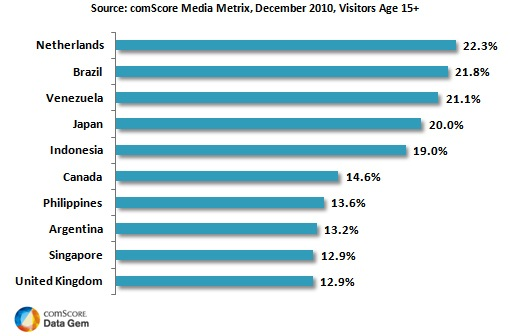
\includegraphics[width=0.472\textwidth, trim=15px 40px 13px 30px, clip]{./resources/twitterglobalmarkets.jpg}
      \label{fig:twitterglobalmarkets}}
    \qquad
    \subfloat[][Facebook covers the majority of people in several countries~\cite{comScoreFacebook}.]{
      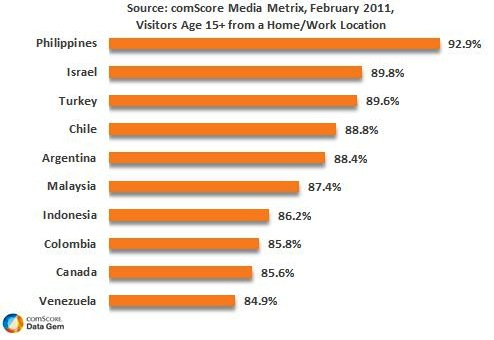
\includegraphics[width=0.458\textwidth, trim=18px 40px 10px 24px, clip]{./resources/facebookglobalmarkets.jpg}
      \label{fig:facebookglobalmarkets}}
\caption{A~significant percentage of the online population participates in social networks.}
\label{fig:globalmarkets}
\end{figure*}

\subsection{Positioning of our Work}
What, to the best of our knowledge, all publications so far have in common is their focus on the author side: it is very well researched what people \emph{produce} on social networks (especially Twitter), whom they follow or unfollow and why, what they tag, whom they put in what list, group, or circle, etc.
However, few to no focus has been put on what people \emph{consume} -- or at least no such study is publicly available.
This is especially true \emph{across} social networks.
As far as we can tell, no study has compared \emph{reader} behavior on \emph{different} social networks in parallel before.
In this work, we thus compare topics people read about on Facebook and on Twitter, and classify those topics in order to provide an overall comparison. 
We therefore have implemented two similar browser extensions: Twitter Swarm NLP\footnote{Twitter Swarm NLP: \url{http://bit.ly/twitterswarmnlp}} and Facebook Swarm NLP\footnote{Facebook Swarm NLP: \url{http://bit.ly/facebookswarmnlp}}. 
On the one hand, these extensions enrich the user experience on the two social networks Facebook and Twitter, and on the other hand, they determine the topics that people see and read about on their timelines by means of named entity disambiguation.
We combine this knowledge with additional anonymous data that we obtain about social network users through Web analytics software.

\subsection{Focus on Desktop Browser Versions}
The two implemented browser extensions require a desktop browser in order to work.
Whenever a user visits a social networking site, in the concrete case Facebook or Twitter, the particular extension gets activated.
By focusing exclusively on content people see when directly navigating to the desktop versions of either \url{twitter.com} or \url{facebook.com} -- therefore on purpose neglecting all activity via applications on \emph{both} desktop and mobile devices -- we assume people indeed read that content.
This is justified by each site's requirement to manually click a link ``$\mathit{n}$ new stories'' (Facebook) or ``$\mathit{n}$ new tweets'' (Twitter) rather than auto-updating the timeline.
Other approaches to determine whether a micropost has been read are limited to microposts with contained Web links and checking whether clicks on those links have occurred.
However, automatic crawling and indexing of links adds hard to detect noise.
We therefore argue that our approach has a higher precision, at the cost of less recall.

\subsection{Paper Objective and Structure}
We outline our paper objectives and non-objectives explicitly, where  each objective has a corresponding non-objective in the two lists below.

\noindent In this paper, we \textbf{will}:
\begin{itemize}
	\item perform analyses based on disambiguated named entities;
	\item perform analyses based on IP-based reader location detection;
	\item work with a manageable amount of microposts read by a random population of social network users;
	\item focus on the micropost reader side.
\end{itemize}
On the contrary, we \textbf{will not}:
\begin{itemize}
	\item perform analyses based on hashtags, term frequencies, or trends;
	\item perform analyses based on geotagged microposts;
	\item work with huge amounts of microposts from ``fire hose'' APIs;
	\item focus on the micropost author side,
\end{itemize}
which is why we strive for a paradigm shift that promises new insights for tasks like brand analysis, opinion research, but also sociological questions.

The remainder of this paper is structured as follows.
\autoref{sec:implementation} focuses on structuring and consolidating unstructured textual micropost data, and introduces browser extensions and Web analytics software.
\autoref{sec:userdemographics} explains our experiment setup and gives an overview of user demographics.
\autoref{sec:discussion} starts with a presentation of raw statistic, then provides a ranking of named entities and gives a categorization of the RDF types of the named entities.
The Section ends with some scenarios from recent history where we show how our approach can be used to reveal new insights that would not be possible with traditional social media mining.
We report on related work in \autoref{sec:relatedwork}, and give an outlook on future work in \autoref{sec:futurework}.
We close the paper with a conclusion in \autoref{sec:conclusion}.

\section{Implementation} \label{sec:implementation}
We have implemented two browser extensions to cover the social networking sites Facebook and Twitter.
These extensions were freely released on a Web store for browser extensions with the following description (slightly adapted):
\begin{quotation}
This extension performs Named Entity Extraction (NEE) on the microposts you read and write on \{Twitter, Facebook\}.
If you write: ``Had froyo for breakfast.'', a named entity would be ``froyo''.
In the sense of Linked~Data, we identify such named entities via a URI, for example \url{http://dbpedia.org/resource/Frozen_yogurt} in the concrete case.
You can see the extracted entities highlighted in each status message \emph{(see \autoref{fig:screenshots})}.
In addition to that, the extracted entities are then reported to a shared Web analytics account via event tracking code  that allows us to build a ranking of the most-talked-about entities.
\end{quotation}
The extensions were released for the Google Chrome browser, the Web Analytics software that we used was Google Analytics.
Micropost texts are sent to a~server that performs named entity extraction.
Afterwards, the original text is discarded and only the extracted entities remain on the server for analysis.

\begin{figure*}
  \centering
    \subfloat[][Twitter Swarm NLP]{
      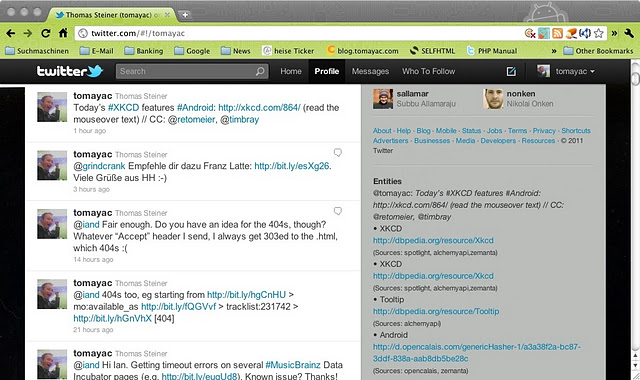
\includegraphics[width=0.47\textwidth,trim=255px 50px 45px 60px,clip]{./resources/twitterswarmnlp.jpg}
      \label{fig:twitterswarmnlp}}
    \qquad
    \subfloat[][Facebook Swarm NLP]{
      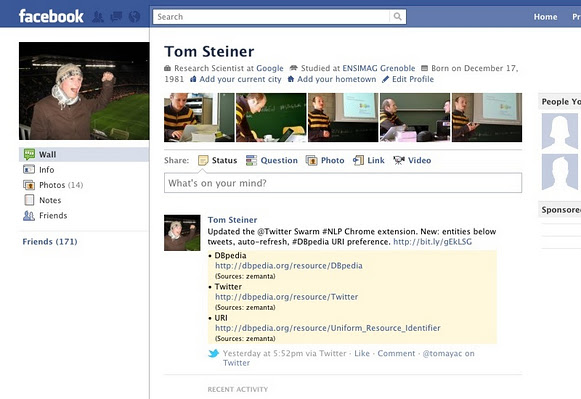
\includegraphics[width=0.45\textwidth,trim=165px 50px 70px 60px,clip]{./resources/facebookswarmnlp.jpg}
      \label{fig:facebookswarmnlp}}
\caption{The two browser extensions in action, displaying the in-page named entity extraction.}
\label{fig:screenshots}
\end{figure*}

\subsection{Structuring Unstructured Data} \label{sec:services}
\textit{A priori}, microposts are unstructured textual data.
We apply so-called Linked~Data rules in order to convert this unstructured data into structured data.
In a first step, the process consists of named entity detection via Natural Language Processing (NLP), and in a second step, named entity disambiguation.
Sir Tim Berners-Lee has introduced Linked~Data in a W3C Design Issue~\cite{TimBL:LinkedData}, where he defines the four rules for Linked~Data as follows:
\begin{enumerate}
\item Use URIs as names for things.
\item Use HTTP URIs so that people can look up those names.
\item When someone looks up a URI, provide useful information, using the standards (RDF*, SPARQL).
\item Include links to other URIs, so that they can discover more things.
\end{enumerate}
In order to represent extracted named entities from microposts in an unambiguous way, we apply the first and the second Linked~Data principle by representing disambiguated named entities with HTTP URIs.
We outsource this task to third party named entity disambiguation Web services (APIs), namely OpenCalais~\cite{OpenCalais}, Zemanta~\cite{Zemanta}, DBpedia Spotlight~\cite{Spotlight}, and AlchemyAPI~\cite{AlchemyApi}.
These APIs take a text fragment as an input, perform named entity extraction and disambiguation on it, and then link the extracted named entities back into the Linking Open Data (LOD) cloud~\cite{LODcloud}.
We use these APIs in parallel, and, by combining their results, aim at the emergence effect in the sense of Aristotle: \emph{``[\ldots] the totality is not, as it were, a mere heap, but the whole is something besides the parts [\ldots]''}\footnote{Aristotle, Metaphysics, Book H 1045a 8-10.}. 

\subsection{Combining Results from Different APIs} \label{sec:consolidation-nlp}
We have implemented a wrapper API for the four named entity disambiguation APIs introduced in \autoref{sec:services} that returns results in JSON format.
While the underlying APIs return entities with their types and/or subtypes, names, relevance, and links into the LOD cloud in different formats, the wrapper API abstracts away the different output formats and returns a common JSON object structure instead.
The JSON output for the exemplary micropost \textit{``Tom has the LaTeX, BibTeX, LaTeX, LaTeX blues...''} can be seen in \autoref{lst:nlpjson}.
The more APIs agree on a disambiguated named entity, the higher the confidence that (i)~the named entity was extracted correctly, and (ii)~the named entity was also disambiguated correctly.
While  in the concrete example ``LaTeX'' and ``blues'' were both correctly extracted and disambiguated (\url{http://dbpedia.org/resource/LaTeX} and \url{http://dbpedia.org/resource/Blues}), the judgment is\linebreak based on just one API result in both cases\linebreak (DBpedia Spotlight and Zemanta respectively),
whereas ``BibTeX'' was correctly extracted and disambiguated (\url{http://dbpedia.org/resource/BibTeX}) by two APIs at the same time (both DBpedia Spotlight and Zemanta).
Hence, the confidence is higher in the latter case.

\begin{lstlisting}[caption={Example JSON output of the named entity disambiguation wrapper, showing different entities and sources.},label={lst:nlpjson}]
[
    {
        "name": "LaTeX",
        "uris": [
            {
                "uri": "http://dbpedia.org/resource/LaTeX",
                "source": "spotlight"
            }
        ],
        "source": "spotlight"
    },{
        "name": "BibTeX",
        "uris": [
            {
                "uri": "http://dbpedia.org/resource/BibTeX",
                "source": "zemanta,spotlight"
            }
        ],
        "source": "zemanta,spotlight"
    },{
        "name": "blues",
        "uris": [
            {
                "uri": "http://dbpedia.org/resource/Blues",
                 "source": "zemanta"
            }
        ],
        "source": "zemanta"
    }    
]
\end{lstlisting}

\subsection{Manipulating Web Pages with Browser Extensions}
Our approach is based on browser extensions.
Browser extensions are small software programs written in a combination of HTML, JavaScript, and CSS.
For this paper, we focus on extensions based on so-called content scripts.
Content scripts are JavaScript programs that run in the context of Web pages via dynamic code insertion.
By using the standard Document Object Model (DOM), they can read or modify details of the Web pages a user visits.
The advantage of using browser extensions is that the concept is very powerful and generalizable at the same time.
Powerful in the sense that it allows for significantly changing one's user experience with social networking sites like Facebook or Twitter and simply adding new features.
Generalizable in the sense that the approach is extensible to more social networking sites like MySpace~\cite{MySpace}, LinkedIn~\cite{LinkedIn}, Google+~\cite{GooglePlus}, etc. in the future.

\subsection{Gathering Visitor Data with Web Analytics Software}
In order to gather high-level information on Web page visitors (apart from low-level log file statistics), so-called Web analytics software can be used.
Such software is typically implemented by adding an invisible snippet of JavaScript code on the to-be-tracked pages of a website.
This code then collects visitor data through requests for a specific $\mathit{1} \times \mathit{1}$ transparent GIF image, also called Web beacon, that is hosted on a Web analytics server.
During these requests, the page and user data is reported in the query part of the Web beacon's URL.
In addition to that, the JavaScript snippet usually sets a first party cookie on a visitor's computer in order to store anonymous information such as the timestamp of the current visit, whether the visitor is a~new or returning visitor, and the referrer of the website that the visitor came from.
Part of the shared visitor information is the IP address, which allows for IP-based geolocation.

\section{Experiment Setup and User Demographics} \label{sec:userdemographics}
\subsection{Experiment Setup}
%We have released the two browser extensions independently from each other for free on a Web store for browser extensions. 
We initially announced the availability of the extensions via Twitter, Facebook, and our personal blog.
Accumulated click statistics for the announcement links are available via the link shortener service bitly\footnote{Statistics: \url{https://bitly.com/elP5OW+} (Facebook Swarm NLP) and \url{https://bitly.com/eBsjQu+} (Twitter Swarm NLP)}.
The extension descriptions contain full disclosure on the collected data and on the usage of a Web analytics tool, however, do not include a concrete mention (apart from a vague remark on entity ranking), that we use the collected data for an experiment.
In addition to that, the extension descriptions do not cross-reference each other, i.e., users are \emph{not} actively encouraged to install both extensions in order to guarantee maximum independence of the experiments.

\subsection{User Demographics} 
As the extensions insert a Web analytics tracking snippet, exact user localization is possible based on the users' current physical location, i.e., completely independent from the origin location users might have registered with Facebook or Twitter, and not to be confused with geotagged microposts.
% A graphical overview of user locations as detected via IP-based geolocation can be seen in Figures~\ref{fig:twitterlocations} and~\ref{fig:facebooklocations}.
Tables~\ref{tab:twitterlocations} and~\ref{tab:facebooklocations} show the distribution of the top-10 locations of extension users. 
The complete statistics can be found \mbox{online}\footnote{Complete statistics: \url{https://github.com/tomayac/swj-microposts/tree/master/stats}}.

\begin{comment}
\begin{figure*}
  \centering
    \subfloat[][Twitter Swarm NLP]{
      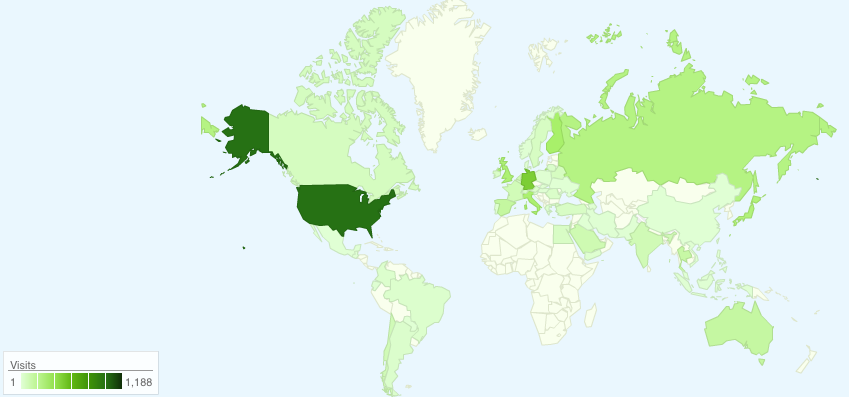
\includegraphics[width=0.47\textwidth, trim=190px 0px 5px 0px, clip]{./resources/twitterlocation.png}
      \label{fig:twitterlocations}}
    \quad
    \subfloat[][Facebook Swarm NLP]{
      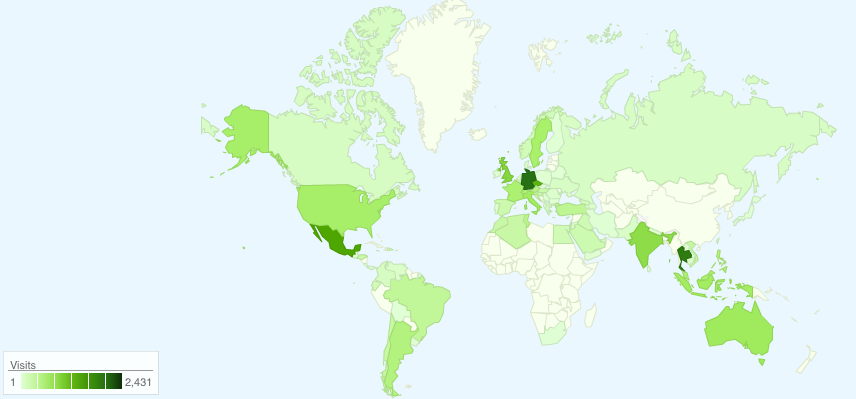
\includegraphics[width=0.47\textwidth, trim=190px 0px 5px 0px, clip]{./resources/facebooklocation.png}
      \label{fig:facebooklocations}}
\caption{Location of users of the two browser extensions (May~1 -- November~12).}
\label{fig:location}
\end{figure*}
\end{comment}

\begin{table*}
  \centering
  \subfloat[][Twitter Swarm NLP.]{
    \begin{tabular}{ | l | l |}
    \hline
	\textbf{Country} & \textbf{Visits} \\ \hline
	United States & 831 \\ \hline
	Japan & 296 \\ \hline
	Germany & 288 \\ \hline
	Italy & 284 \\ \hline
	Finland & 204 \\ \hline
	United Kingdom & 200 \\ \hline
	Australia & 176 \\ \hline
	Russia & 162 \\ \hline
	Thailand & 155 \\ \hline
	Spain & 147 \\
    \hline
  \end{tabular}
  \label{tab:twitterlocations}}
  \qquad
  \subfloat[][Facebook Swarm NLP.]{
    \begin{tabular}{ | l | l |}
    \hline
	\textbf{Country} & \textbf{Visits} \\ \hline
	Germany	& 2,280 \\ \hline
	Thailand & 2,133 \\ \hline
	Mexico & 1,586 \\ \hline
	Czech Republic & 1,416 \\ \hline
	United Kingdom & 1,100 \\ \hline
	India & 1,047 \\ \hline
	Australia & 854 \\ \hline
	Indonesia	& 826 \\ \hline
	Italy & 805 \\ \hline
	United States & 742 \\
    \hline
  \end{tabular}
  \label{tab:facebooklocations}}
  \tablecaption{An analysis of the top-10 locations of the browser extensions' users exposes a~varied geographical pattern.}
  \label{tbl:locations}
\end{table*}

In the period from March~1 to November~8, for the Facebook Swarm NLP, overall \emph{858~unique Facebook users} accessed the extension at least 10~times, in comparison to overall \emph{86~unique Twitter users} for the Twitter Swarm NLP.
If we put these figures in contrast to the \emph{seven~day~active users} statistics for the extensions (Figures~\ref{fig:facebookswarmnlpstats} and~\ref{fig:twitterswarmnlpstats}), where the Facebook Swarm NLP reached~135, and the Twitter Swarm NLP~72 \emph{seven~day~active users} as of November~6, we can derive that overall relatively few Twitter users installed the extension and stayed with it for the whole time of the experiments, whereas overall relatively many Facebook users installed the extension, used it for a short while, and then uninstalled it.

\begin{figure*}
  \centering
    \subfloat[][Twitter Swarm NLP]{
      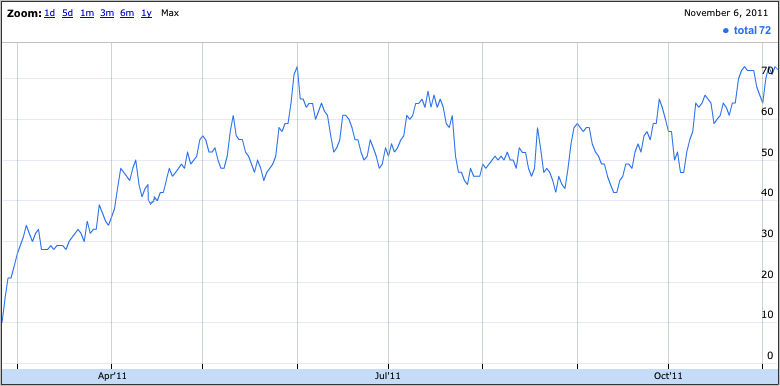
\includegraphics[width=0.47\textwidth, trim=3px 2px 3px 20px, clip]{./resources/twitterswarmnlpstats.png}
      \label{fig:twitterswarmnlpstats}}
    \quad
    \subfloat[][Facebook Swarm NLP]{
      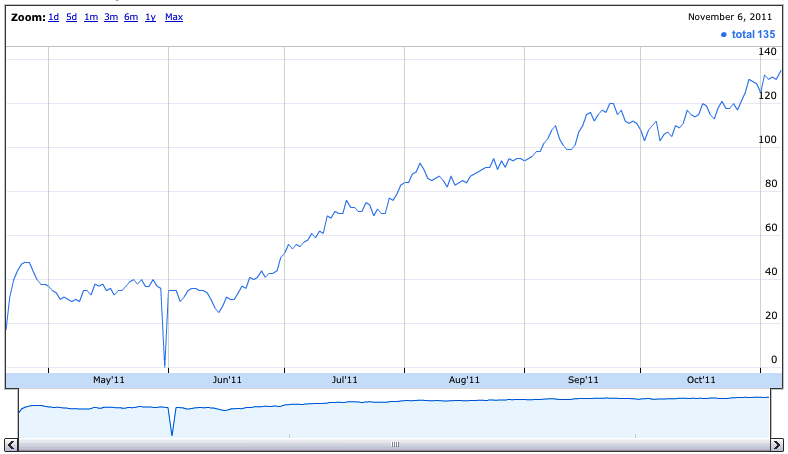
\includegraphics[width=0.47\textwidth, trim=3px 2px 3px 20px, clip]{./resources/facebookswarmnlpstats.png}
      \label{fig:facebookswarmnlpstats}}
\caption{The seven~day~active user count for both extensions follows a~stable or slowly increasing trend.}
\label{fig:swarmnlpstats}
\end{figure*}

\section{Discussion} \label{sec:discussion}
In this Section, we delve into the collected data, which ranges over more than six months.
We cover the period from May~1 to November~12, 2011.
It is to be noted that our data, while \emph{not} statistically significant, shows promising trends and potential direction for future research.
If in the following we present results, those are to be taken with a grain of salt.
However, common sense suggests that they are correct.
The experiments were conducted over more than six months, which reduces the risk of short-term spikes.

\subsection{Raw Statistics} \label{sec:rawstatistics}
First, we present some raw statistics on both social networking sites.
\autoref{tbl:raw} shows the absolute, total, and unique number of occurrences of named entities from microposts.
Interesting here is especially the relation between \emph{unique} named entities and \emph{total} named entities.
To clarify the difference between unique and total named entities, we consider the following examples.
In a~first case, one user during one social networking session reads two different microposts that contain one common named entity (e.g., two consecutive Facebook posts that talk about cats).
Here, we would track two total named entities, but only one unique named entity.
In a second case, two different users during their social networking session read two different microposts that contain one common named entity. Here, we would still track two total named entities, however, also two unique named entities.
In short, a unique named entity is a named entity that during one social networking session of one user appears only once.
The number of absolute named entities refers to the absolute distinct number of named entities that ever occurred during the experiments, independent from users and sessions.

Looking at the numbers, where we have 76.7\% unique named entities for Twitter and 43.0\% unique named entities for Facebook, we can carefully derive that the reading experience per social networking session on Twitter is more versatile than on Facebook.
We need to note, however, that Facebook microposts are generated at a lot lower frequency than Twitter microposts, and that Twitter microposts are limited to 140 characters, which may have an impact on both precision and recall of the named entity disambiguation process.
The average duration of a visit on Facebook according to our statistics is 66~min.\ against 28~min.\ on Twitter, which implies that Twitter users spend less than half the time than Facebook users on their social networking site.
Again, our data is at this point \emph{not} statistically significant, especially as we had the interesting phenomenon of almost more than ten times as many absolute distinct Facebook users than Twitter users.
However, \emph{seven~day~active user} statistics show only about double the number of Facebook users (see \autoref{sec:userdemographics}).
Further research is necessary that takes the following factors into account:
\begin{itemize}
\item \emph{Micropost length and effect on recall and precision of named entity disambiguation.}
Rizzo \textit{et al.} provide first results in this direction~\cite{nerd}.
\item \emph{Throughput of microposts per time unit (smaller than one day) and effect on versatility of unique named entities per social networking session.}
This stands in an interesting contrast to the number of absolute distinct named entities, which is significantly higher on Facebook.
\item \emph{Steadiness of the group of experiment participants over time.}
The key point of our approach was that participants were unaware that they were contributing to an experiment.
We were surprised that so many Facebook users participated, albeit for a short period of time, whereas so few Twitter users participated, however, in the majority during the whole time.
\item \emph{Increase reach through focusing on more browser platforms.}
Currently we have limited ourselves to one browser platform, however, the approach can be applied to all browser platforms that support extensions or plug-ins.
\end{itemize}

\begin{table*}
  \centering
    \begin{tabular}{|l | r | r | r | c | c |}
    \hline
    \textbf{Network} &
	\textbf{Absolute} & \textbf{Total} & \textbf{Unique} & \textbf{Unique / Total (\%)} & \textbf{Avg. Visit Length} \\ \hline
	\textbf{Twitter} &
	18,207 & 35,958 & 27,594 & 76.7\% & 00:28:12 \\
    \hline
    \textbf{Facebook} &
	54,331 & 316,910 	& 136,196 & 43.0\% & 01:06:07 \\ 
    \hline
  \end{tabular}
  \tablecaption{Twitter users relatively read more distinct entities than Facebook users do.\\* However, Facebook sessions take generally longer, which may account for this difference.}
  \label{tbl:raw}
\end{table*}

\subsection{Ranking of Named Entities}
The core outcome of our experiments is a comparison of the named entities on the social networking sites Facebook and Twitter.
From the absolute distinct number of 18,207 (Twitter) and 54,331 (Facebook) of named entities, we have manually cleaned the list of the top-200 named entities on each social network, removed false positives, and normalized the representing URIs to DBpedia URIs.
This was done by inspecting the extracted entities and the words they correspond to in the Analytics tool.
In \autoref{fig:topentities}, we present the remaining list of top entities for each social network.
Visually, the curves are very similar with five named entities occurring many times, and then a long tail of many named entities occurring few times.

\begin{figure*}
  \centering
    \subfloat[][Twitter Swarm NLP.]{
      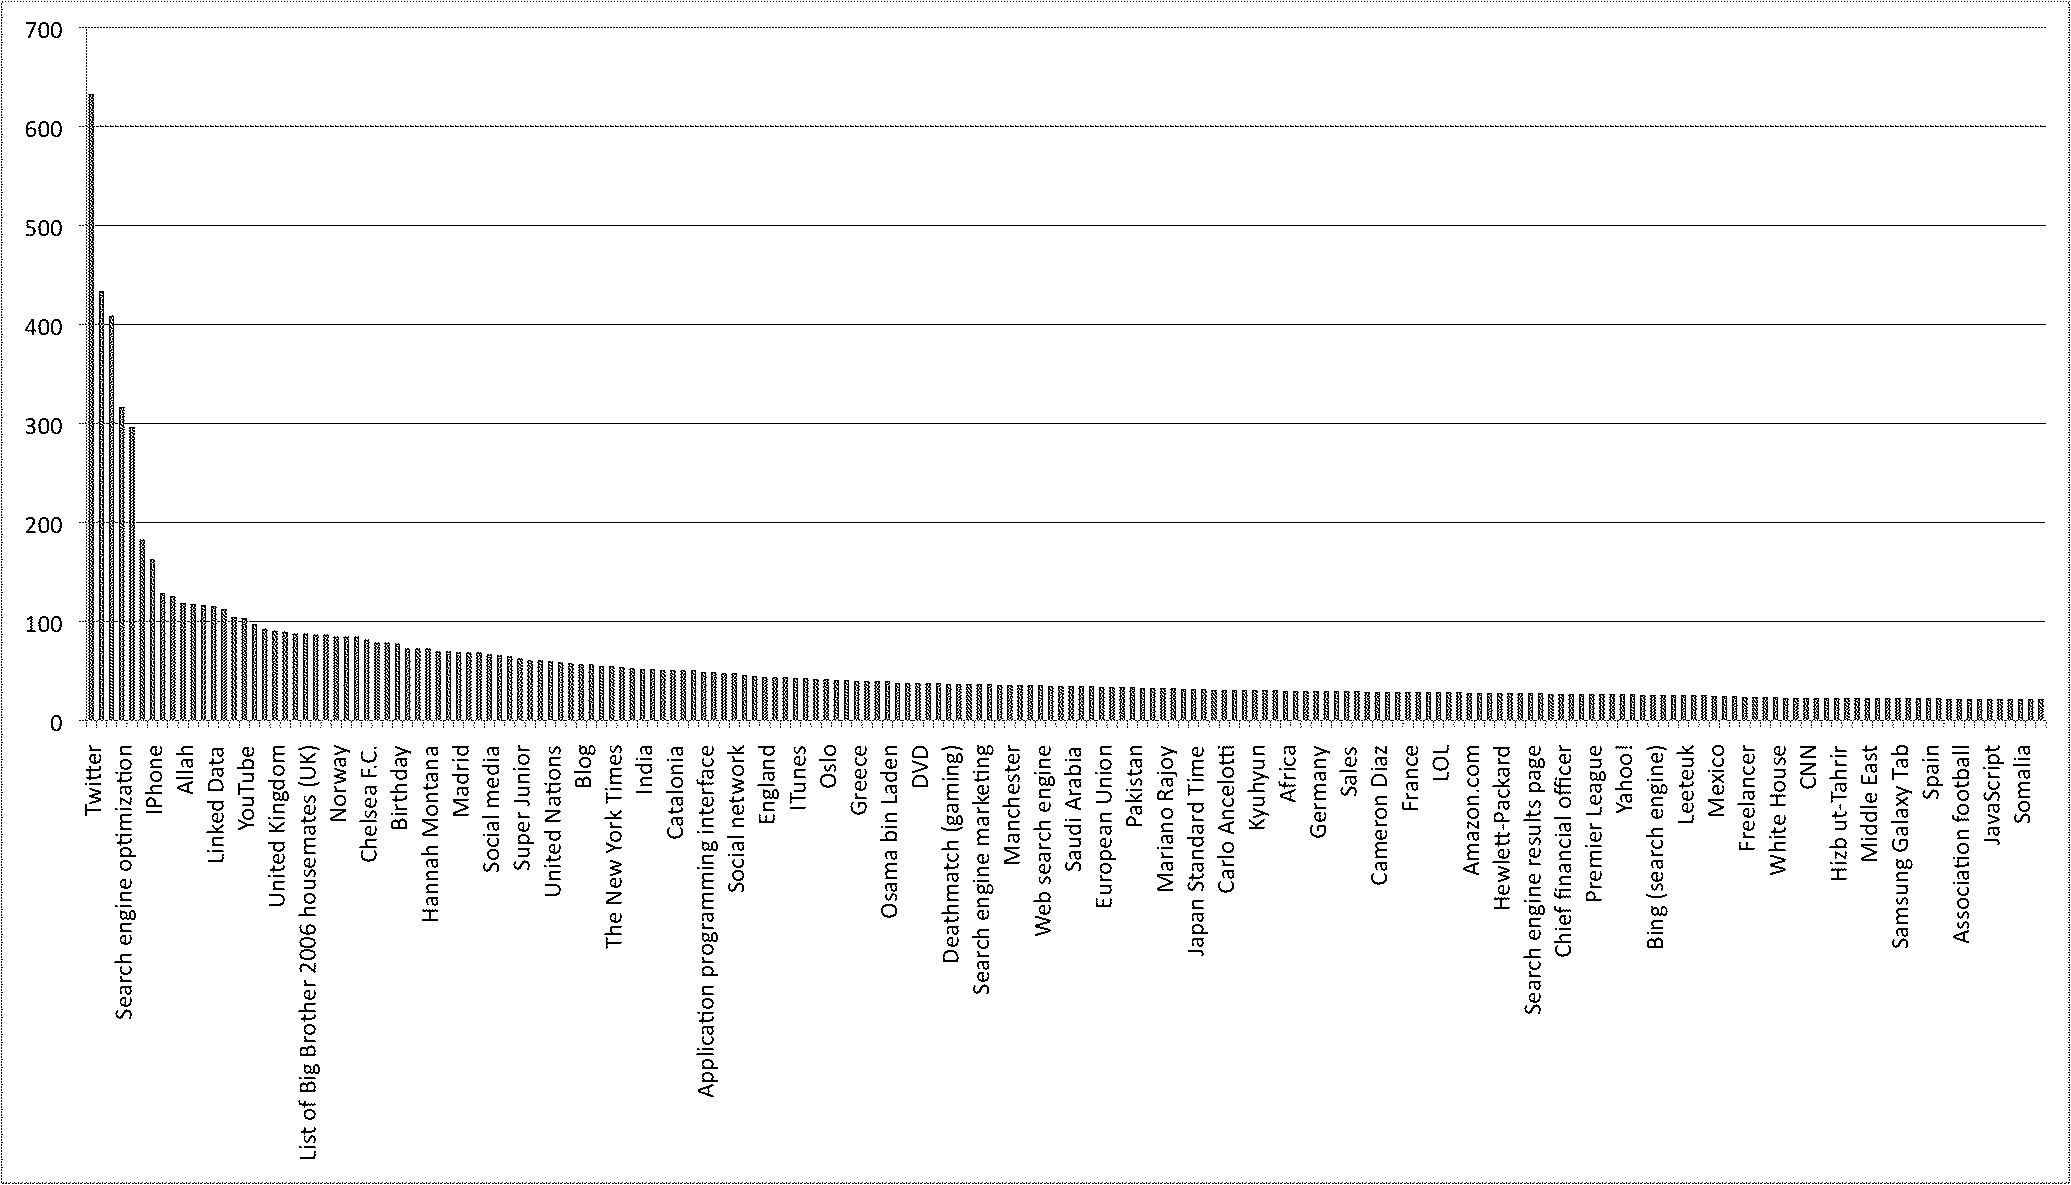
\includegraphics[width=\textwidth, trim=4px 4px 4px 4px, clip]{./resources/twittertopentities.png}
      \label{fig:twittertopentities}}
    \qquad
    \subfloat[][Facebook Swarm NLP.]{
      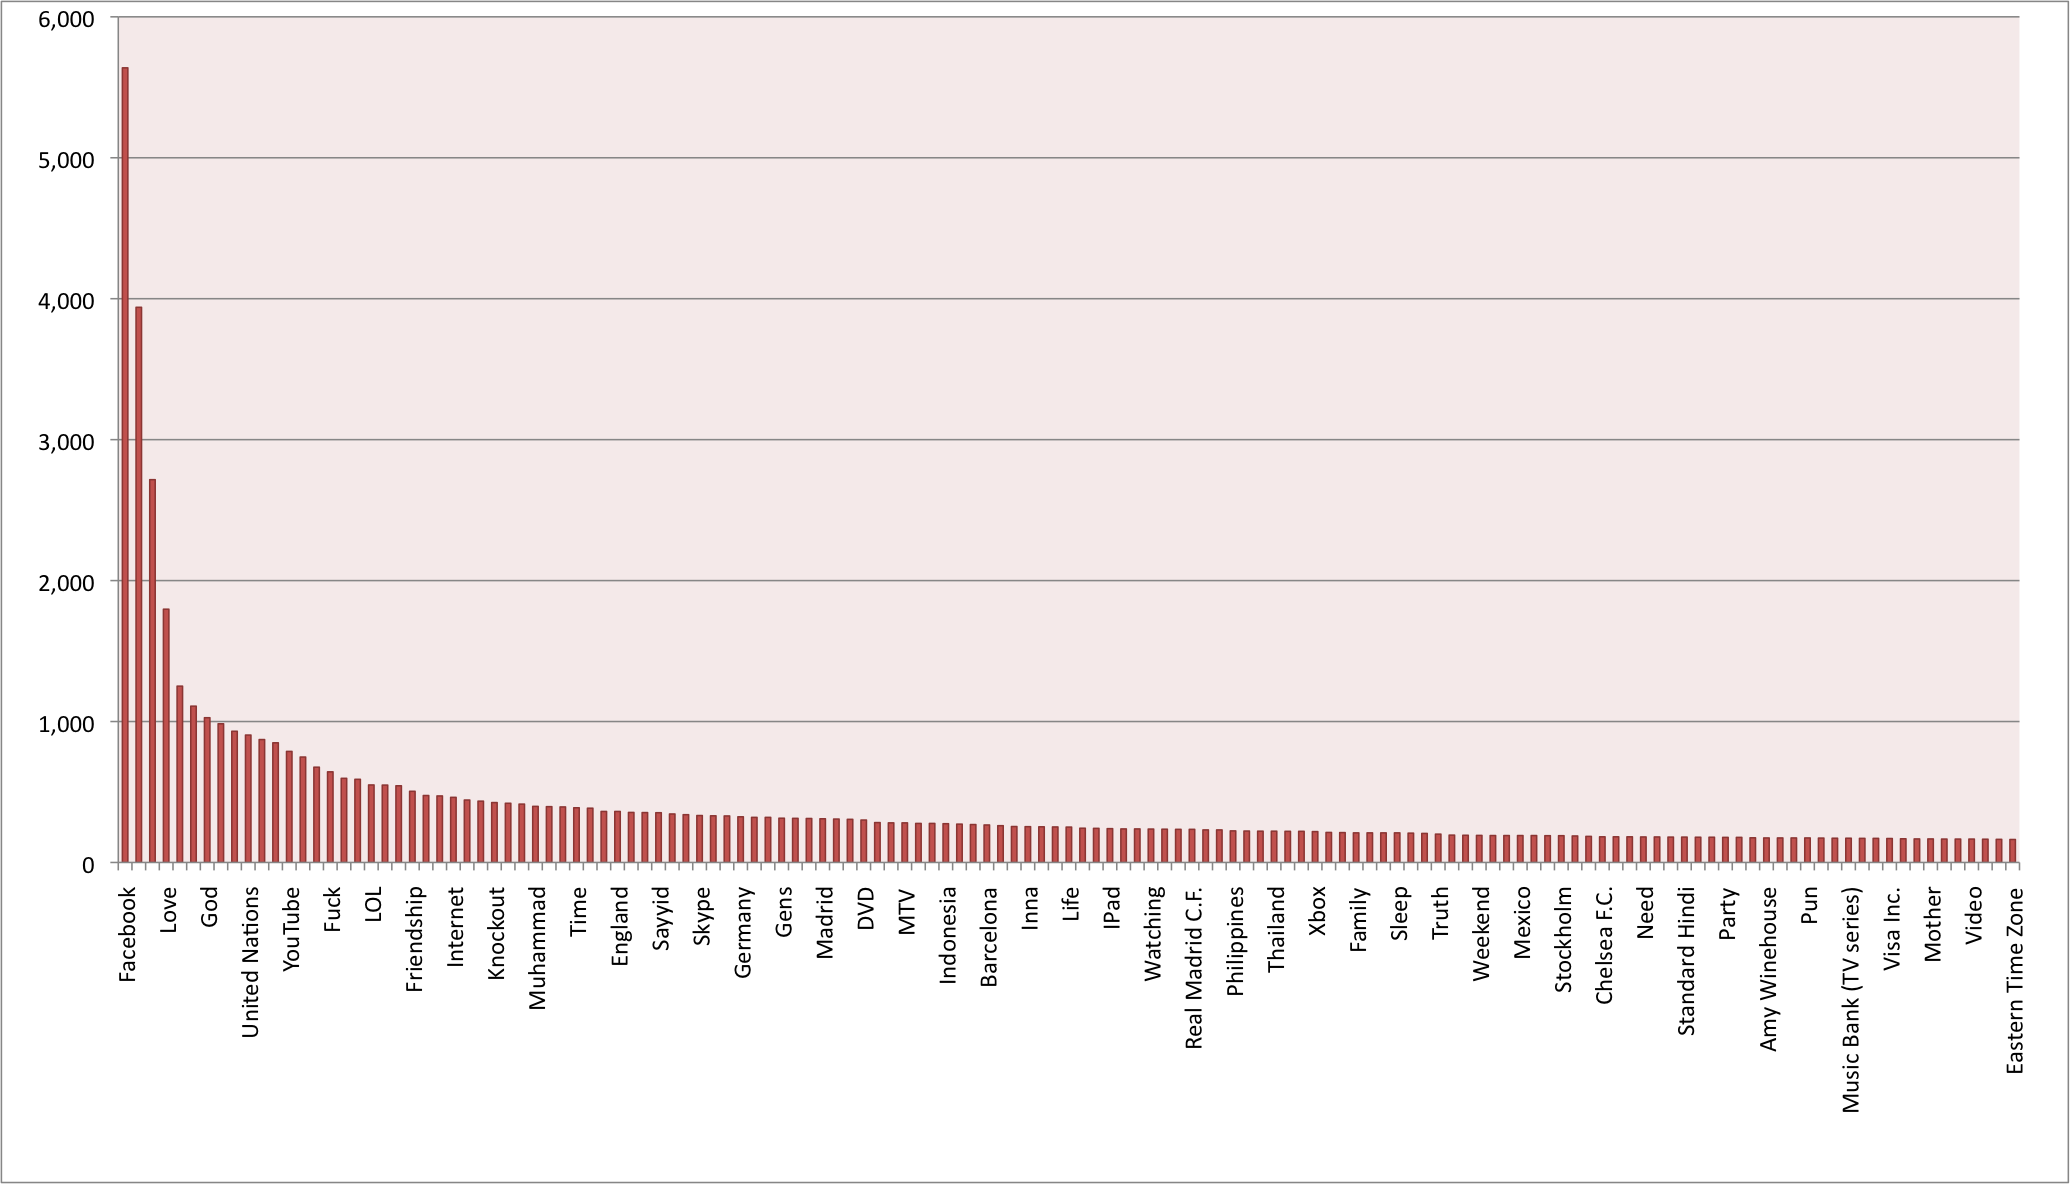
\includegraphics[width=\textwidth, trim=4px 4px 4px 4px, clip]{./resources/facebooktopentities.png}
      \label{fig:facebooktopentities}}
\caption{The top entities reported by both browser extensions follow a~Zipf distribution with a~high peak and a~long tail.}
\label{fig:topentities}
\end{figure*}

\autoref{fig:top10} zooms in on just the top-10 entities.
Interesting to note is the top named entity on each social network, which is the particular social network name ``Twitter'' and ``Facebook'' itself. 

\begin{figure*}
  \centering
    \subfloat[][Twitter users tend to read technical stories.]{
      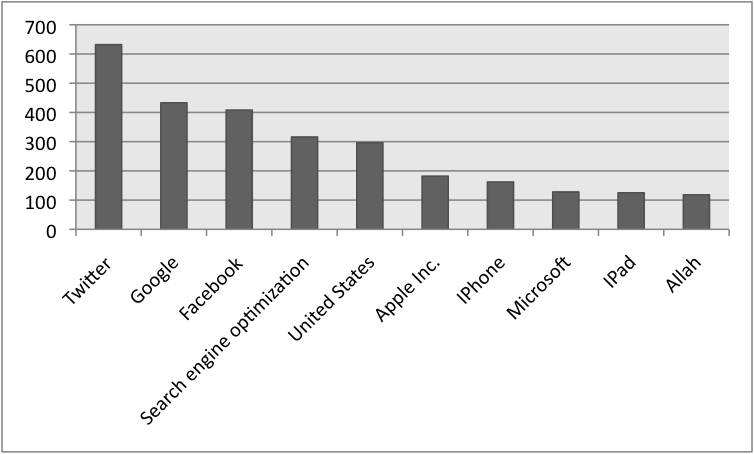
\includegraphics[width=0.45\textwidth, trim=2px 10px 2px 2px, clip]{./resources/twittertop10.png}
      \label{fig:twittertop10}}
    \qquad
    \subfloat[][Facebook users tend to read personal stories.]{
      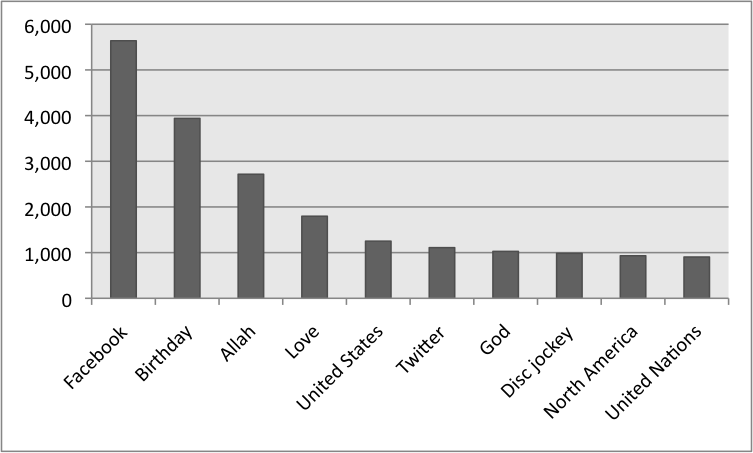
\includegraphics[width=0.45\textwidth, trim=2px 10px 2px 2px, clip]{./resources/facebooktop10.png}
      \label{fig:facebooktop10}}
\caption{The top-10 consumed entities for both networks clearly show a~subject bias.}
\label{fig:top10}
\end{figure*}

On Twitter, five out of the top-10 named entities are IT-related companies, namely ``Twitter'', ``Google'', ``Facebook'', ``Apple'', and ``Microsoft''.
Two Apple products, the ``iPhone'' and the ``iPad'' hold the positions 7 and 8.
``Search engine optimization'' (SEO) holds position 4, the ``United States'' of America are on 5, and position 10 is held by ``Allah''.
Interpreting these results, we can say that 8 out of the top-10 named entities on Twitter by reader interest are of technical nature.

On Facebook, the second most read about named entity is ``birthday'' on position 2.
Position 3 is held by ``Allah'', who is followed by the (Christian) ``God'' on position 7.
``Love'' is on position 4.
As the sole company, ``Twitter'' appears on position 6.
The ``United States'' of America and ``North America'' are on positions 5 and 9 respectively.
The ``disc jockey'' (DJ) spins a hit single on position 8.
Finally, the political organization ``United Nations'' holds position 10.
If we interpret the results, Facebook is used most for personal matters like reading social network friends' birthday felicitations, reading about love and relationships, but also religious matters of Islamic and Christian nature.
Music plays a significant role on Facebook, reflected by the presence of disc jockey.
With regards to reader interest, there is a tendency towards reading about the United States, or North America in general.

\subsection{Segmentation by RDF Type}
One of the advantages of using DBpedia URIs to represent named entities in an unambiguous way is that the Linked~Data knowledge from DBpedia can be leveraged.
Therefore, we have retrieved the RDF type (\texttt{rdf:type}) information for the top-500 named entities for both networks,
after a~manual cleaning operation.
Unlike the main DBpedia OWL type (\texttt{dbpedia-owl:type}), the \texttt{rdf:type} can have multiple values, for example a company can be both a company, and an organization.
Type specifications can come from different namespaces, like \texttt{dbpedia-owl} (\url{http://dbpedia.org/ontology/}), \texttt{yago} (\url{http://dbpedia.org/class/yago/}), or \texttt{umbel} (\url{http://umbel.org/umbel/rc/}).

\begin{figure*}
  \centering
    \subfloat[][Twitter]{
      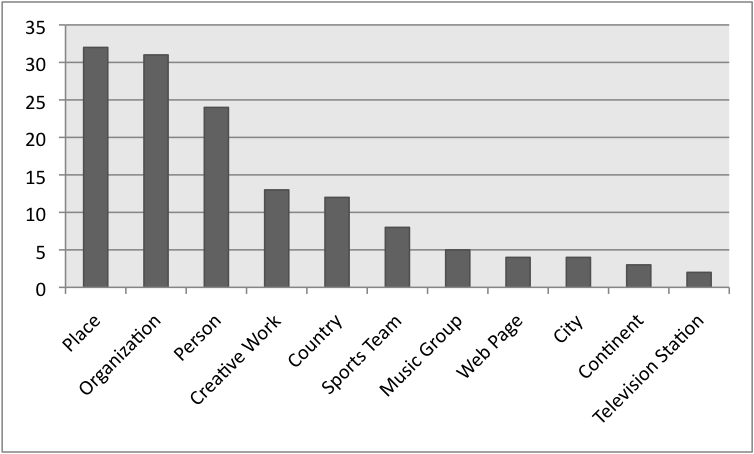
\includegraphics[width=0.48\textwidth, trim=10px 5px 5px 5px, clip]{./resources/twitterschema.png}
      \label{fig:twitterschema}}
    \subfloat[][Facebook]{
      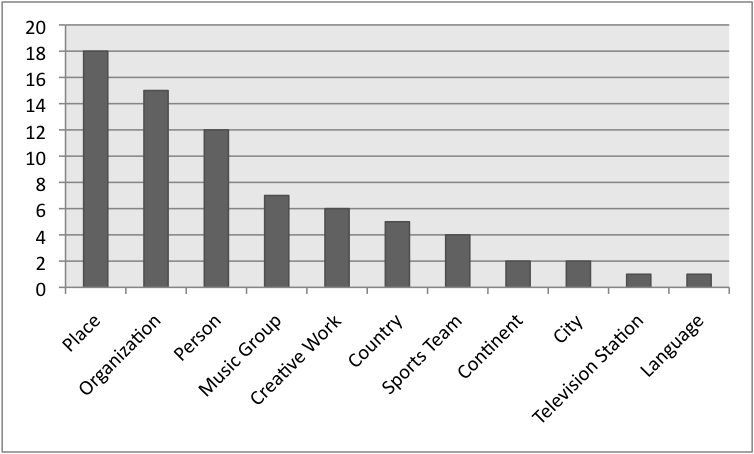
\includegraphics[width=0.48\textwidth, trim=10px 5px 5px 5px, clip]{./resources/facebookschema.png}
      \label{fig:facebookschema}}
\caption{The six-month entity type statistics also follow a~Zipf distribution, wherein a~few types have many occurrences, and many types have few occurrences. Displayed here are schema.org types, but the same observation can be made for all ontologies and their combinations.}
\label{fig:schema}
\end{figure*}

A recent addition is the \texttt{schema} namespace \url{http://schema.org/} around the common schema effort of the big search engines Google, Yahoo!, and Microsoft~\cite{schemaorg}.
The difference lies in the granularity of the underlying ontologies.
For example, where \texttt{schema} just has ``Place'', \texttt{umbel} differentiates between ``Location'' and ``Populated Place''.
Applying a loose ontology mapping, the top-3 types on both social networks are Place, Organization, Person for \texttt{schema} and \texttt{dbpedia-owl}, and Place, Organization, Business for \texttt{umbel}.
\autoref{fig:schema} shows the distribution of the types of the most common named entities within the observation period, clearly illustrating the long tail of type specifications.

\subsection{Events from Recent History}
\label{subsec:RecentEvents}
In this Subsection, we present some events from recent history and show how, using our approach, new insights or trends can be revealed.

\subsubsection{Facebook Reader Perception of the 2011 Norway Attacks}
On July 22, a mass shooting took place on the island of Utøya in Norway, preceded by a car bomb explosion in Oslo\footnote{2011 Norway attacks: \url{http://en.wikipedia.org/wiki/2011_Norway_attacks}}.
We start our analysis with a deep-dive into the most read about named entities in Norway on the day of the attacks and then manually filter the list for relevance to the event.
\autoref{tab:norway} shows the resulting \mbox{top-6} ranking of named entities on July 22 on Facebook.
The list is led by the two geographic entities of the city of ``Oslo'' and the country of ``Norway''.
Ranks 3 to 5 are held by traditional news media: the popular newspaper ``Verdens Gang'', typically just referred to as VG, the Cable News Network ``CNN'', and the ``Norwegian Broadcasting Corporation'', known as NRK.
The current Norwegian Prime Minister ``Jens Stoltenberg'' follows on rank 6.
It is interesting to note how Norwegian readers got detailed information on the attacks through local media (VG and NRK), but also through the international company CNN.
Traditional media companies more and more harvest social networking sites for authentic coverage of events.
For Utøya, this is documented, e.g., in the case of survivor Adrian Pracon (@AdrianPracon on Twitter) in a tweet from Sky News producer @fimackiesky\footnote{Sky News contact Utøya survivor: \url{https://twitter.com/\#!/AdrianPracon/status/94573763500326912}}.
While Facebook has terminated terrorist Anders Behring Breivik's profile, the Internet already has conserved a copy\footnote{Copy of the terrorist's Facebook profile: \scriptsize\texttt{http://} \texttt{publicintelligence.net/mirror-of-utøya-gunman-anders} \texttt{-behring-breiviks-facebook-page-and-photo-gallery/}}. 

\textbf{Revealed insight:}
traditional news media still play the most important role in informing people, albeit the news item itself is shared via social networks. 

\begin{table}
    \begin{tabular}{ | l | l |}
    \hline
	\textbf{Named Entity} & \textbf{Total (in Norway)}\\ \hline
	db:Oslo & 75\\
	db:Norway & 57\\
	db:Verdens\_Gang & 42\\
	db:CNN & 19\\
	db:Norwegian\_Broadcasting\_Corporation & 18\\
	db:Jens\_Stoltenberg & 16\\
    \hline
  \end{tabular}
  \tablecaption{The above entities where the most present in user's perception on the 2011 Norway attacks (July~22).}
  \label{tab:norway}  
\end{table}

\subsubsection{Comparison of Reader Geolocations for the Arab Spring}
The Arab Spring is a revolutionary wave of demonstrations and protests occurring in the Arab world\footnote{Arab Spring: \url{http://en.wikipedia.org/wiki/Arab_Spring}}.
We compared sub continent geolocations of readers of microposts mentioning the countries of Egypt, Libya, and Syria on both Facebook and Twitter.
The results for both social networks can be found in \autoref{tab:arabspring}.
First, it is interesting to note the sequence of the countries.
On Twitter, it is Libya, Egypt, and Syria, whereas on Facebook it is Egypt, Libya, and Syria. 
Reader sub continent geolocation distribution is different as well.
Where on Facebook the Western European region is most interested in the three countries, on Twitter it is the Northern African region.
From Twitter users in Northern Africa, Egypt was the most read about country, in contrast to the among global Twitter users more popular Libya.
Overall, the Arab Spring was almost equally represented on both social networks, albeit our numbers are only sufficient for trend analyses.
Both social networks play an important role for the organization of the protests and the distribution of eyewitness statements.

\textbf{Revealed insight:}
comparing reader geolocations to distinguish geographic centers of interest can be especially useful to detect local social networking preferences.

\begin{table*}
  \centering
  \subfloat[][Twitter]{
    \begin{tabular}{ | l | l | l | l | l | l | l |}
    \hline
    & \textbf{Total} & \textbf{Northern Africa} & \textbf{Southern Europe} & \textbf{Northern Europe} & \textbf{Northern America} & \textbf{Australia and New Zealand}\\ \hline
    \textbf{db:Libya} & 104 & 1 & 38 & 33 & 16 & 9\\
    \textbf{db:Egypt} & 86 & 47 & 22 & 0 & 5 & 10\\
    \textbf{db:Syria} & 69 & 17 & 5 & 8 & 15 & 12\\
    \hline
    \end{tabular}
  \label{tab:twitterarabspring}}  
  \qquad
  \subfloat[][Facebook]{
    \begin{tabular}{ | l | l | l | l | l | l | l |}
    \hline
	 & \textbf{Total} & \textbf{Western Europe} & \textbf{Northern Africa} & \textbf{Australia and New Zealand} & \textbf{Northern Europe} & \textbf{South-Eastern Asia}\\ \hline
	\textbf{db:Egypt} & 128 & 41 & 47 & 11 & 13 & 3\\
	\textbf{db:Libya} & 68 & 20 & 20 & 12 & 0 & 5\\
	\textbf{db:Syria} & 61 & 23 & 9 & 15 & 1 & 5\\
    \hline
  \end{tabular}
  \label{tab:facebookarabspring}}
    \tablecaption{Sub continent geolocations of reader interest of some of the Arab Spring key countries (May~1 -- November~12).}
  \label{tab:arabspring}
\end{table*}

\subsubsection{Brand Popularity on City Level on Facebook}
Celcom Axiata Berhad, DBA Celcom, is the oldest mobile telecommunications company in Malaysia\footnote{Celcom: \url{http://en.wikipedia.org/wiki/Celcom}}.
We show the brand's popularity based on named entity occurrences pivoted by cities of readers interested in micropost mentioning the company.
\autoref{tab:celcom} shows the top-5 cities where people read about Celcom.
This allows for targeted brand awareness campaigns in cities where the brand has a low popularity, potentially based on additional sentiment analysis.

\textbf{Revealed insight:}
City level analyses allow for fine-grained details on, e.g., brand popularity over time.

\begin{table*}
    \begin{tabular}{ | l | l | l | l | l | l | l |}
    \hline
	& \textbf{Total} & \textbf{Shah Alam} & \textbf{Kuching} & \textbf{Kuala Lumpur} & \textbf{Keningau} & \textbf{Kulim}\\ \hline
\textbf{db:Celcom} & 173 & 47 & 34 & 18 & 16 & 16\\
    \hline
  \end{tabular}
  \tablecaption{Popularity of the Celcom brand on city level (May~1 -- November~12).}
  \label{tab:celcom}  
\end{table*}

\subsubsection{LOLcats vs. LOLdogs on Facebook}
One of the more popular Internet phenomena is the sharing of cute cat and dog photos\footnote{LOLcats: \url{http://en.wikipedia.org/wiki/LOLcat}}.
On November 23, the well-known link shortening service \emph{bitly} published term popularity-based statistics to test the hypothesis that ``kittens really rule the Internet''~\cite{kittens}.
According to their results, dogs clearly outperform cats among all \emph{produced} links on microposts.
With our approach, we were able to confront bitly's results with the \emph{consumed} microposts around cats and dogs on Facebook.
\autoref{tab:kittens} shows that among micropost readers, cats indeed haz rule the Internetz.

\textbf{Revealed insight:}
the importance of differences between producer and consumer sides becomes evident.

\begin{table}
    \begin{tabular}{ | l | l | l |}
    \hline
	\textbf{Named Entity} & \textbf{Total} & \textbf{Unique} \\ \hline
	db:Cat & 161 & 41\\
	db:Dog & 122 & 43\\
	db:Persian\_(cat) &29 &5\\
	db:Kitten & 23 & 7\\
	db:Chihuahua\_(dog) & 9 & 1\\
    \hline
  \end{tabular}
  \tablecaption{Reader popularity of cats and dogs on Facebook\\* (May~1 -- November~24).}
  \label{tab:kittens}  
\end{table}

\section{Related Work} \label{sec:relatedwork}
We report on related work separated into different areas of research:
\begin{itemize}
\item \emph{semantic annotation of microposts}, which focuses on named entity detection and disambiguation;
\item \emph{trend or popularity detection}, which is based on term frequencies;
\item \emph{commercialization of social data}, which aims at monetization of gathered insights.
\end{itemize}
The presented examples are not to be seen as \emph{the} standard selection of relevant work, but rather as representative overview on a plethora of very similar publications and services.
In addition to that, we also provide a \emph{comparison of our work to micropost author-focused approaches}.

\subsection{Semantic Annotation of Microposts}
Passant \textit{et al.} introduced a Semantic MicroBlogging (\textit{sic}) framework (SMOB,~\cite{Passant2008}) that enables a \textit{distributed, open, and semantic} microblogging experience based on Semantic Web and Linked~Data technologies by annotating microposts with common vocabularies such as FOAF or SIOC.
SMOB relies on distributed autonomous hubs that communicate with each other to exchange microposts and subscriptions, which can also be cross-posted to Twitter.
Hashtags, words or phrases preceded by the '\#' symbol, have been popularized on Twitter as a way for users to organize and search messages~\cite{hashtag}.
The authors suggest the use of meaningful hashtags such as \texttt{\#dbp:Eiffel\_Tower} or \texttt{\#geo:Paris\_France}, in the style of widely used RDF prefixes for DBpedia and GeoNames.

In the Linked Open Social Signals project\linebreak (LOSS,~\cite{Mendes:LOSS}), Mendes \textit{et al.} investigate the representation of microposts as Linked Open Data and address the problem of information overload caused by the sheer amount of microposts (the authors call the opinions, observations, and suggestions contained in microposts ``social signals'', hence the project name).
While the micropost community has come up with hashtags in order to categorize microposts, these hashtags are ambiguous and have to be explicitly added to the micropost by the author and due to length constraints are sometimes left out in favor of more text.
The main goal of LOSS is thus to enable collective analysis of social signals for sense-making by using Linked Open Data principles in combination with realtime push models.

\subsection{Trend and Popularity Detection}
As outlined before, research on trend and popularity detection has mainly focused on Twitter due to the facile availability of data through the Twitter Streaming API.
A basic overview is given by by Benhardus in~\cite{benhardus2010streaming}, where the author applies and evaluates several methodologies to large Twitter corpora such as (normalized) term frequency, TF-IDF, and entropy.
With TwitterMonitor~\cite{Mathioudakis:2010:TTD:1807167.1807306}, Mathioudakis and Koudas present a \textit{bursty} keyword-based Twitter trend detector demonstration.
Their algorithm is able to detect groups of bursty keywords and also enrich trends with potentially associated keywords.
Trendsmap~\cite{trendsmap} provides a realtime mapping of Twitter trends across the world.
The service allows for splitting up one's view in different granularity levels by current location, city, region, and world.

What the Trend~\cite{whatthetrend} is a service that provides manually curated and annotated reports on Twitter top-trending topics.
The service adds explanations to why tropics trend and data behind trending patterns.
Primarily, the information on What the Trend is user-generated, however, the service also sells curated yearly reports.

Topsy Labs, Inc. offers a commercial API~\cite{topsy} that allows for \textit{applying social intelligence to realtime decisioning}.
Therefore, the service applies algorithms that try to rank popular videos, photos, blog posts, and news stories, most influential users on a certain topic, and individual user influence scores.
Supported social networks include Twitter and Google+.
Different from the social networks themselves, Topsy Labs claims to allow for going back in history up to the year 2008 with their commercial API.

Twimpact~\cite{twimpact} is a realtime Twitter data analysis company with special focus on social media communication that reports \textit{immediate events, current trends, and relevant opinion leaders} within social media conversations.
Twimpact uses machine learning-based ranking techniques that do not rely on simple reader/follower counts, but rather include actual communication patterns, such as retweets. 

\subsection{Comparison with Micropost Author-focused Approaches} \label{sec:comparison}
With our focus on micropost readers rather than on micropost authors, we strive for a paradigm shift with important consequences.

The first and most important consequence is the availability of only a limited set of micropost data, as illustrated by the Venn diagram in \autoref{fig:vennreadunread}.
Only a subset (of unknown size) of all microposts that get authored also ever gets read, whereof in turn our approach covers an unknown fraction.
Where the Twitter Streaming API offers up to 10\% coverage of all authored tweets, full access to the ``fire hose'' with 100\% coverage of all authored tweets is handled through Twitter data providers~\cite{dataproviders}.
For Facebook, no such publicly available option exists.
For obvious reasons, there is no API from either of the networks for read microposts, which is why we came up with the idea to hook into the reading experience on social networks through browser extensions.
Attracting a~larger amount of users is feasible if sufficient incentives are provided.
For instance, significant extra functionality can be provided on top of the named entity extraction, such as automated micropost summarization to enable a~faster and more broad social media experience.

\begin{figure}
\centering
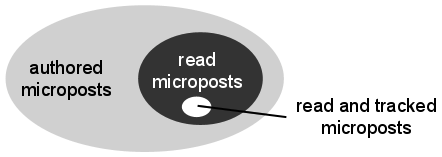
\includegraphics[width=0.6\linewidth]{./resources/vennreadunread.png}
\caption{Only a subset (of unknown size) of all microposts that get authored also ever get read. In turn, we can track only a small subset of all read microposts with our extensions.}
\label{fig:vennreadunread}
\end{figure}

The second consequence has to do with privacy issues.
While aggregated public data made available via APIs may feel like violating privacy~\cite{nyt}, it is still public data.
However, the approach we took in this paper goes one step further by explicitly accessing a social network user's timeline, and reporting back named entities to a Web analytics service (the same that already gets used natively by Twitter). 
It is important to note, however, that no connection is been made between a user's individual timeline and the person behind.
Also, no private conversations are monitored.
We have stated all accessed data in the extension descriptions.

The third consequence is the potential bias introduced by targeting specific Web browsers with the extensions and the willful neglect of desktop and mobile applications. 
With regards to specific Web browsers, for now, we have focused on the Google Chrome browser due to its native Chrome Web Store that guarantees optimal exposure of the extensions in a centralized way.
Concerning desktop and mobile applications, there is definitely some, albeit unmeasurable, bias.
However, unofficial statistics from Twitstat~\cite{twitstat} suggest that the desktop Web version of Twitter is still the means for the majority of its users to access the social network.
For Facebook, official usage statistics~\cite{facebookstats} state that from more than 800 million active users more than 350 million currently access Facebook through their mobile devices, which still means that the majority use Facebook via the desktop Web version.

\section{Future Work} \label{sec:futurework}
A drawback of our approach is that getting statistically significant data is difficult.
The bigger the so-called panel, the more representative the results.
At its core, this is not a new problem.
The television viewership audience measurement system described in~\cite{patent:20100011389} is comparable to our approach:
whenever a viewer switches channels, the system automatically reports a~channel switch event back to a tracking server.
Analogically, whenever a micropost reader reads a micropost, the detected and disambiguated named entities are automatically reported back to the Web analytics software via our browser extensions.
For radio and television audience measurement, a Portable People Meter device~\cite{PortablePeopleMeter} developed by Arbitron is used in some parts of the United States.
We imagine a similar setting for our approach where randomly selected social network users can be asked to participate in micropost audience measurement studies.

In \autoref{sec:rawstatistics} we have outlined factors to be taken into account in order to improve the quality of statistical data.
With the proposed switch to an officially disclosed micropost audience measurement setup, the two last factors, increasing the study reach and the steadiness of the experiment participants, will resolve nicely in the sense of being the same as with traditional audience measurement.

We have already covered the theoretic consequences of the paradigm shift of focusing on the micropost author side in \autoref{sec:comparison}.
More work is needed to practically compare the differences in results with common scenarios like the one proposed in the beginning: \textit{``Is my brand~X more popular in region~R on social network~A, or social network~B?''}.
Evidently, conditions apply, which make the comparison interesting.
The determination of the region~R has to be interpolated with traditional social media mining, whereas our approach has exact IP geolocation-based location awareness.
Reader and author popularity of a brand can be different, and finally, the sample size of the set of examined microposts will be different.

\section{Conclusion} \label{sec:conclusion}
Social networks play a crucial role for all sorts of serious and non-serious questions of life.
This can go as far as regimes censoring social networks altogether, as it has happened in Egypt~\cite{censor}.
While tech-savvy Internet users can circumvent censorship barriers, the general population is effectively cut off of social network communication.
In order to help Egyptians share eyewitness statements about the happenings in their country again, a phone-based \emph{Speak-to-Tweet} service that required no Internet connection was established~\cite{egypt}.
Our approach can help prioritize such anti-censorship efforts by analyzing where reader interest is located geographically, and what social networks people use for their information needs.

This paper, to the best of our knowledge, for the first time, was focused on the consumer point of social media.
Although the amount of data was smaller than with similar, producer-oriented studies, we were able to confirm some interesting differences in social media consumption.
Concretely, the most read Twitter messages are technical in nature, while the most read Facebook updates concern personal matters.
This measuring method promises interesting new aspects for future research, for example, to choose the right social medium for a~certain data mining task.
On the economical side, businesses can use social media consumer behavior to develop advertising strategies, since today, they still depend on producer behavior as a second-degree estimation, or base their decisions on manual and error-prone surveys.

We have presented a generalizable approach towards the comparison of topics people read about on social networks.
We have shown how named entity disambiguation combined with classic Web analytics can be applied to the social networks Facebook and Twitter.
With concrete examples, we have highlighted how the approach of traditional social media mining can be completed and enriched with our reader-focused approach.
We have compared both approaches and worked out the limitations and advantages of both.
The main contribution of the paper is on the one hand the comparison of reader topics of two social networks and the classification of those topics, and on the other hand the paradigm shift contained in the approach itself.
The approach being generalizable, future studies can cover and compare more social networks.

\section*{Acknowledgments}
We would like to thank Shaun Roach from AlchemyAPI, Andraž Tori from Zemanta, Pablo Mendes from DBpedia Spotlight, and Tom Tague from OpenCalais for their precious support and/or generous API quota allowances. 

T. Steiner is partially supported by the European Commission under Grant No. 248296 FP7 I-SEARCH project.
J. Gabarr\'o is partially supported by TIN-2007-66523 (FORMALISM), and SGR 2009-2015 (ALBCOM).
The research activities as described in this paper were funded by Ghent University, the Interdisciplinary Institute for Broadband Technology (IBBT), the Institute for the Promotion of Innovation by Science and Technology in Flanders (IWT), the Fund for Scientific Research Flanders (FWO Flanders), and the European Union.

%%%%%%%%%%% The bibliography starts:
\bibliographystyle{abbrv}
\bibliography{swj2012}

\end{document}
